This page provides a form to create a new course.
Professors can enter the course name and details, and they can specify the weekly time slots for meeting with students.

\begin{figure}[H]
    \centering
    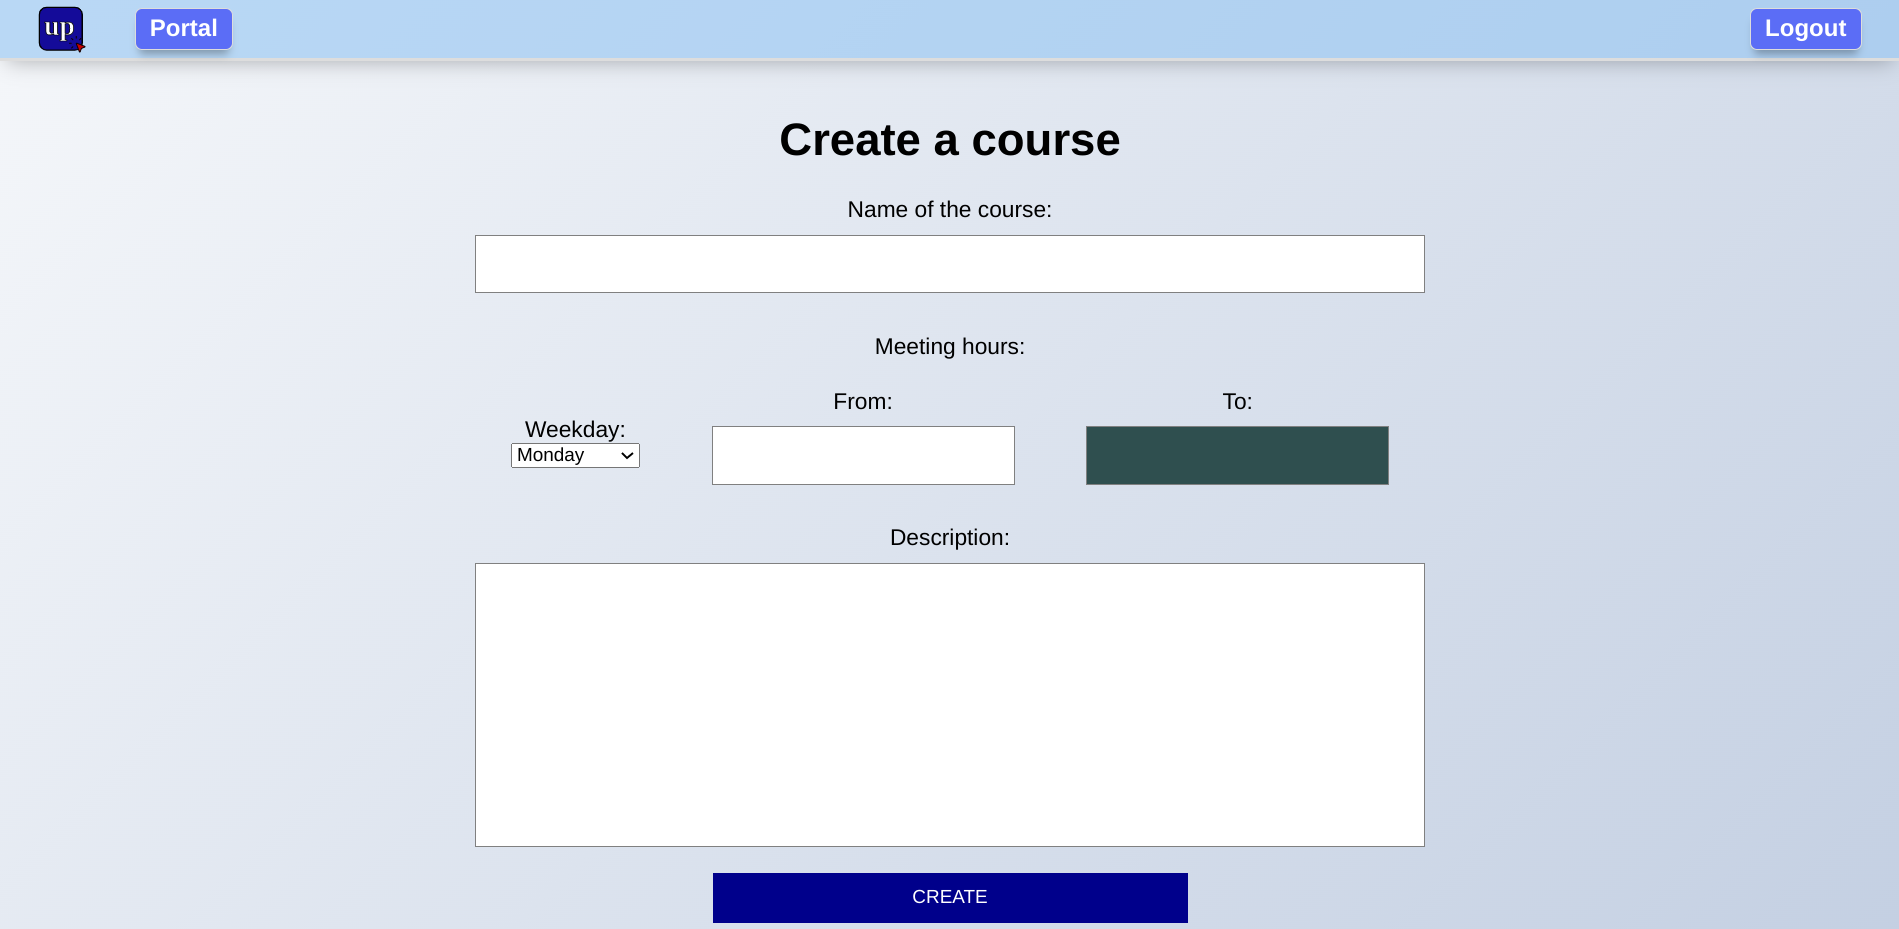
\includegraphics[width=\textwidth]{img/user_manual/professor/create-course-1.png}
    \caption{Screenshot of the course creation page, with an empty form}
\end{figure}

\begin{figure}[H]
    \centering
    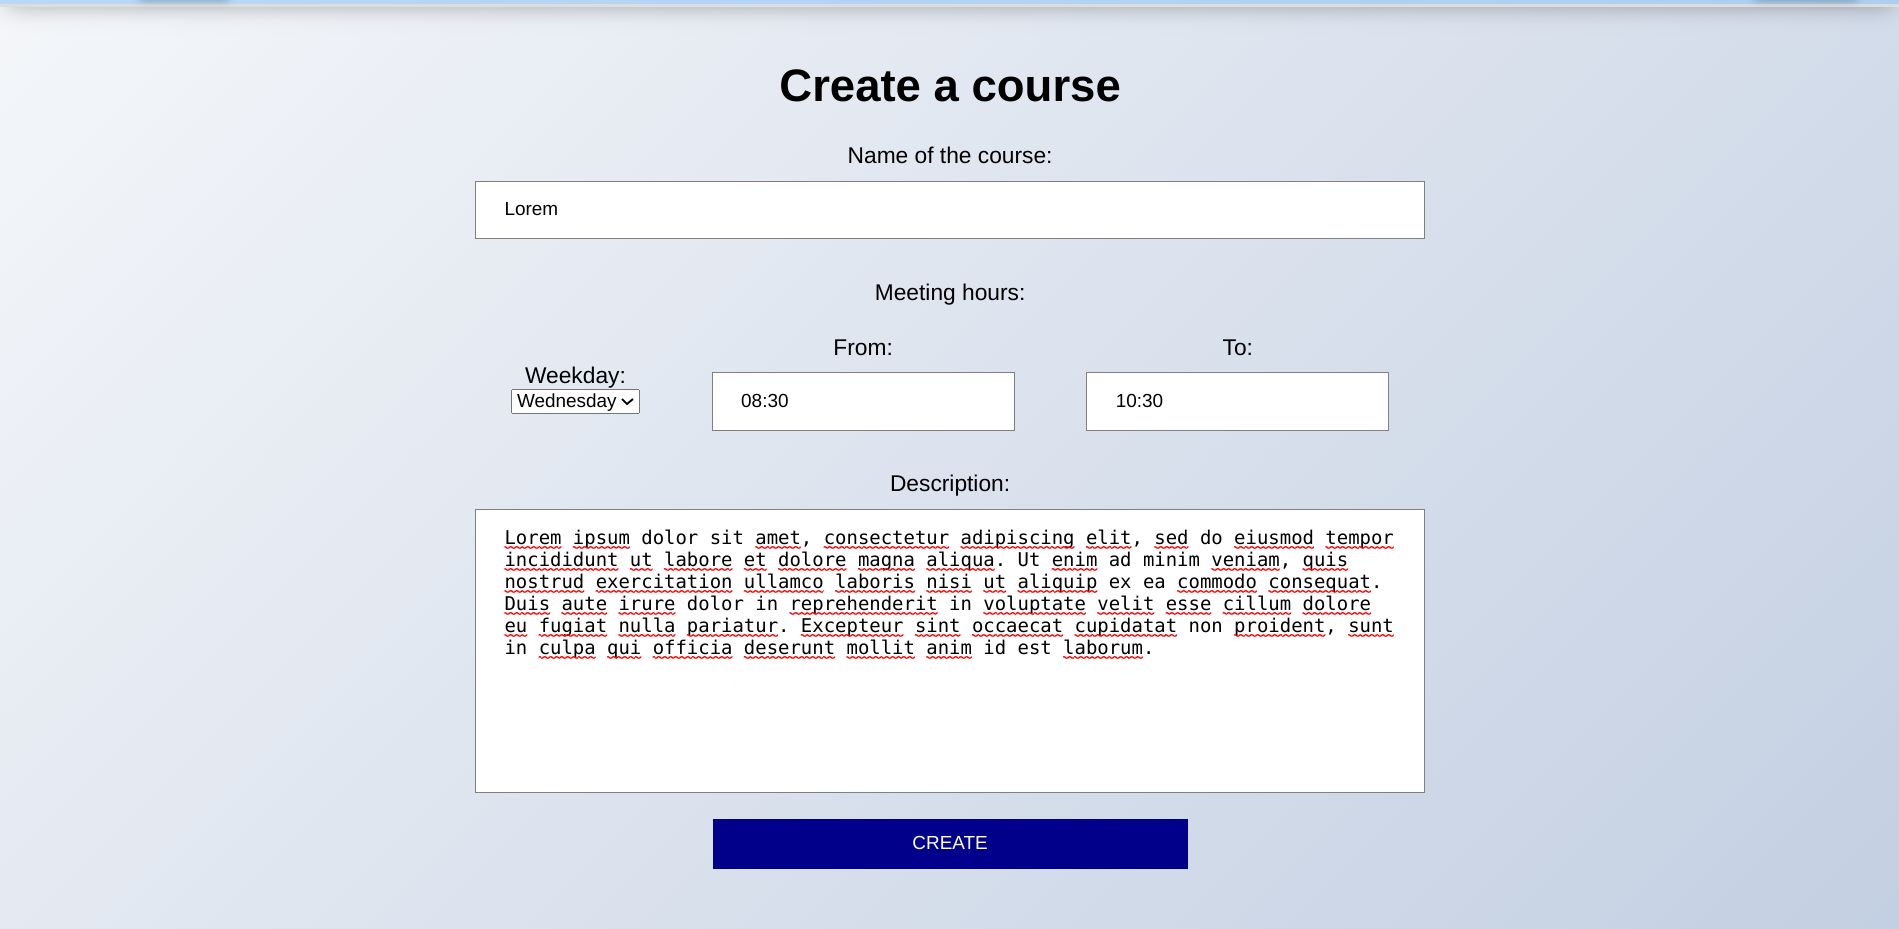
\includegraphics[width=\textwidth]{img/user_manual/professor/create-course-2.png}
    \caption{Screenshot of the course creation page, with a filled form}
\end{figure}

After the professor submits the form, the browser shows an alert pop-up with the result (success/failure) of the course creation.

\begin{figure}[H]
    \centering
    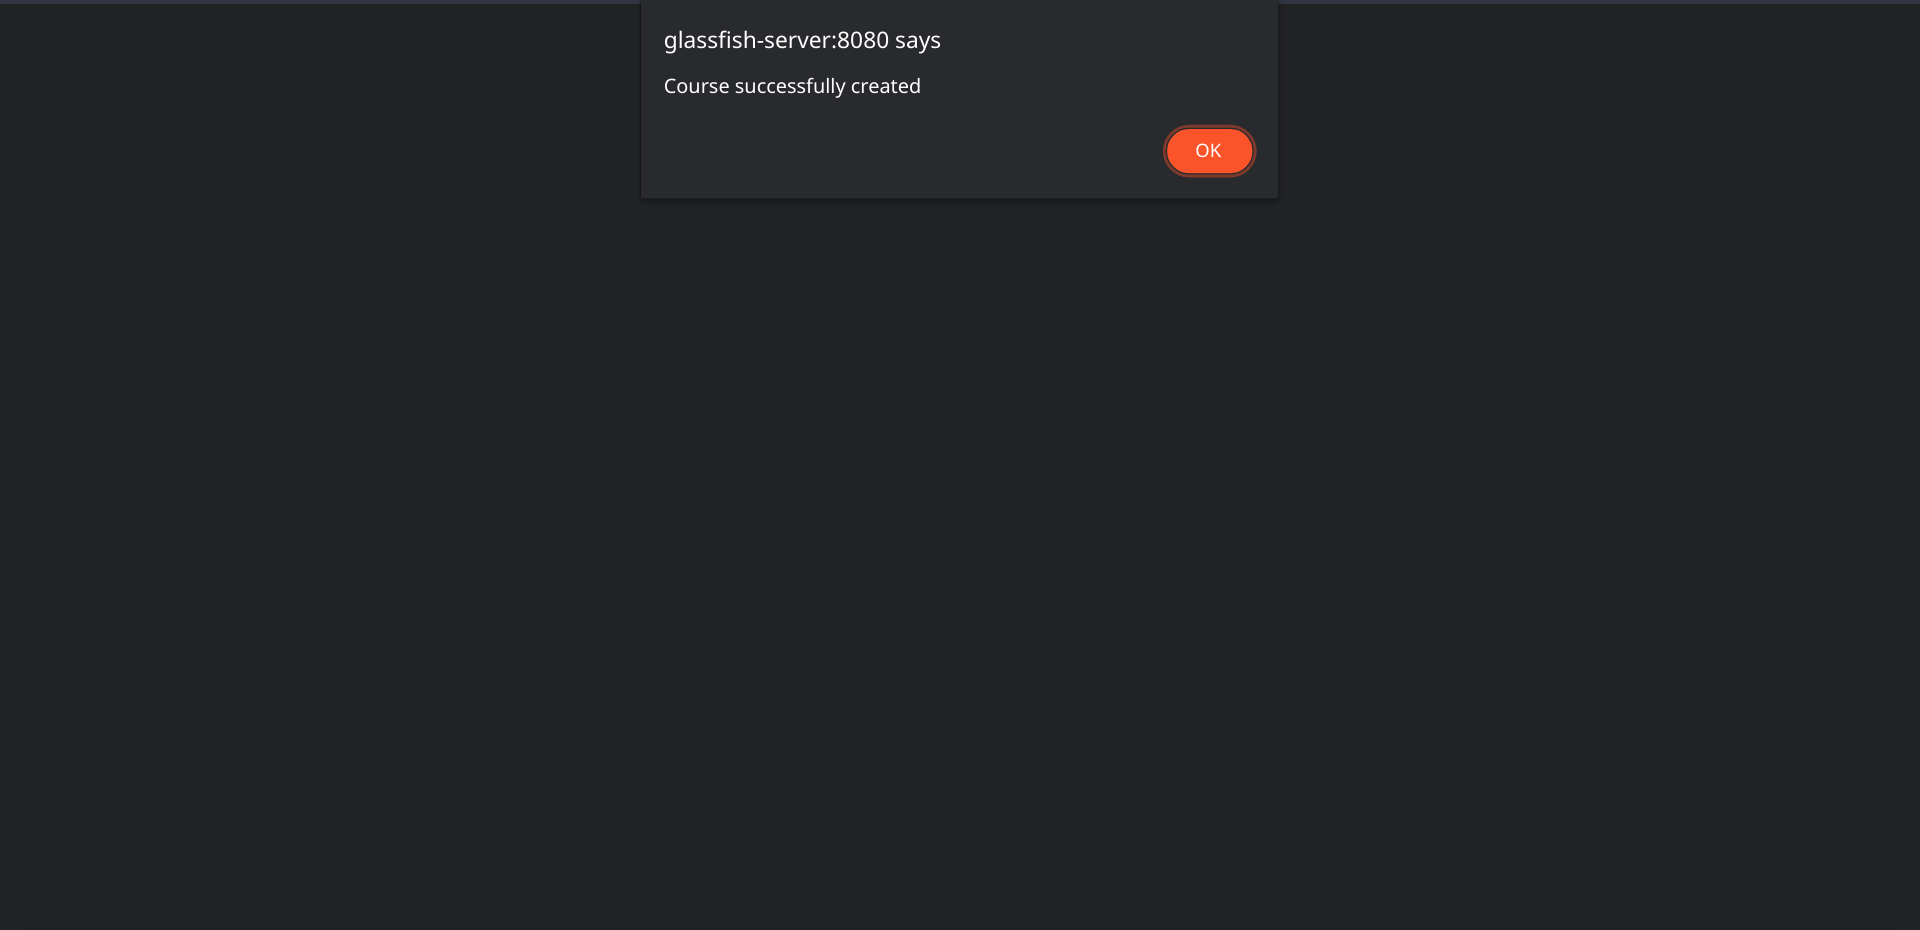
\includegraphics[width=\textwidth]{img/user_manual/professor/create-course-3.png}
    \caption{Screenshot of the course creation page, after the professor submits the form and creation succeeds}
\end{figure}

If the creation succeeds, every student will be able to view the course details page and book a meeting in the available time slots.

\begin{figure}[H]
    \centering
    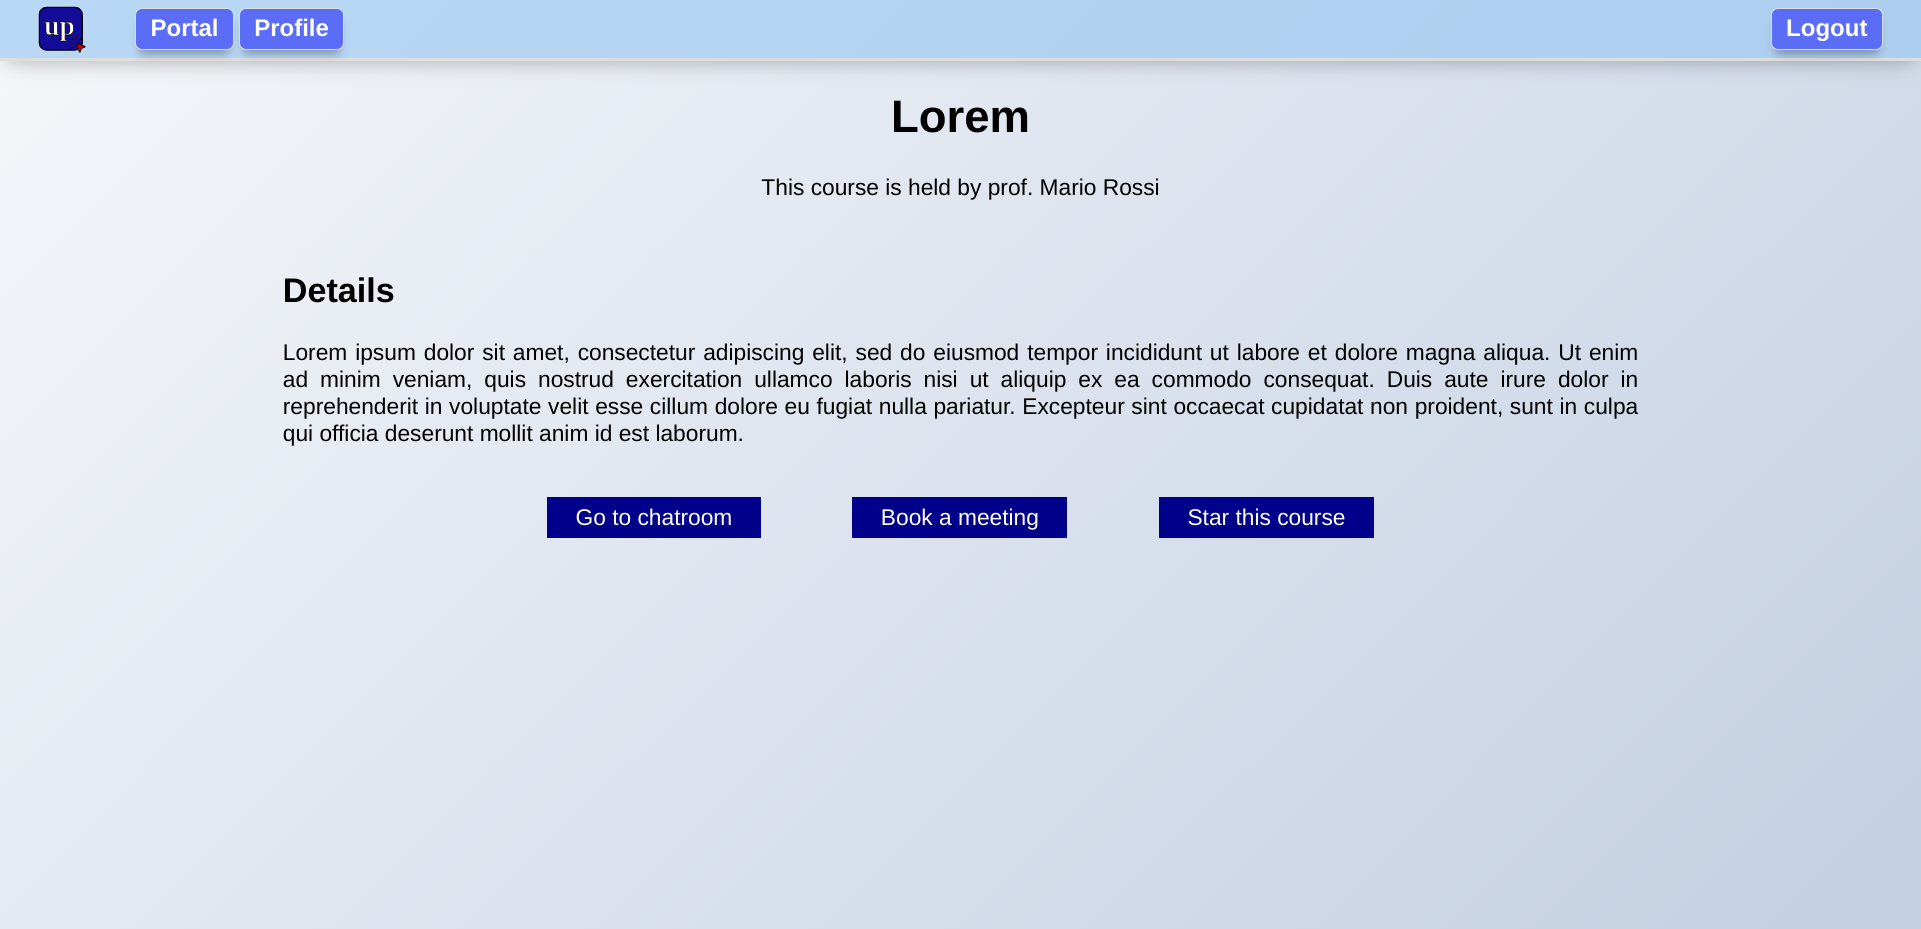
\includegraphics[width=\textwidth]{img/user_manual/professor/create-course-4.png}
    \caption{Screenshot of the course detail page, after the creation of the course}
\end{figure}

\begin{figure}[H]
    \centering
    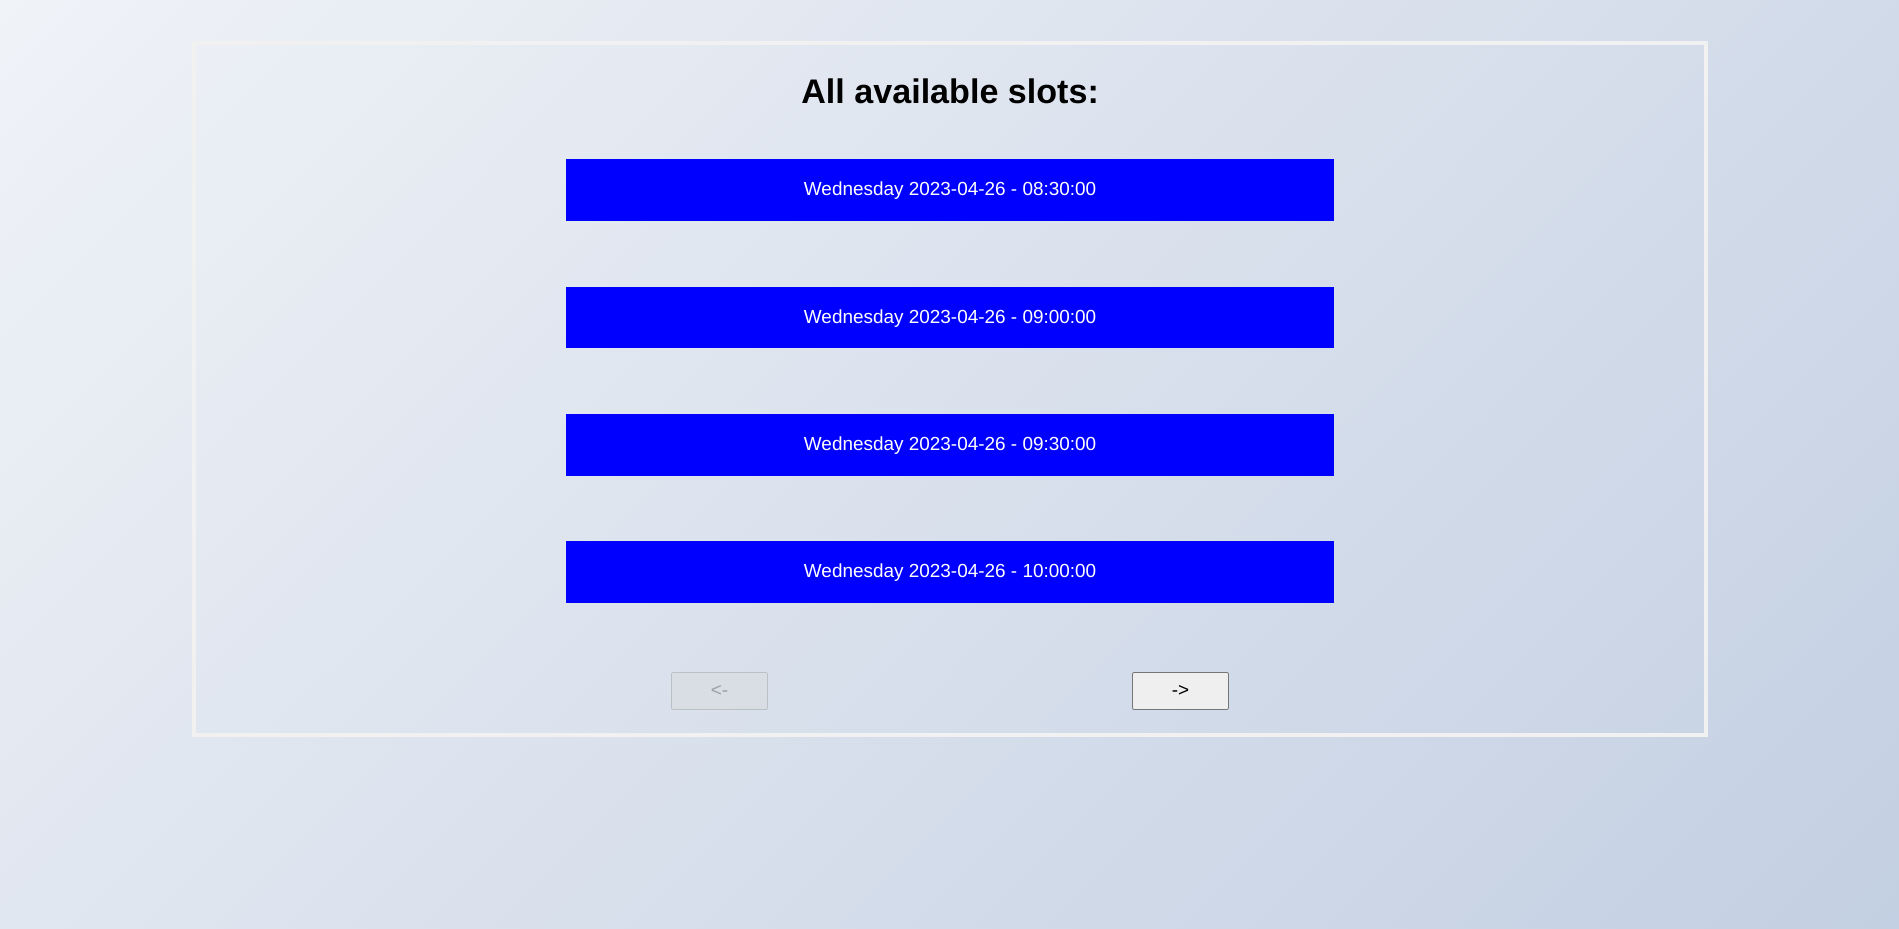
\includegraphics[width=\textwidth]{img/user_manual/professor/create-course-5.png}
    \caption{Screenshot of the page for booking a meeting, after the creation of the course}
\end{figure}

